\onehalfspacing
\section{Đề số 3}
\graphicspath{{./img/}}
\begin{bt} 
    Cho $\mathrm{x}, \mathrm{y}, \mathrm{z}$ là các số khác 0 và $\mathrm{x}^2=\mathrm{yz}, \mathrm{y}^2=\mathrm{xz}, \mathrm{z}^2=\mathrm{xy}$.\linebreak[2]
    Chứng minh rằng: $\mathrm{x}=\mathrm{y}=\mathrm{z}$.
\loigiai{
    Vì $\mathrm{x}, \mathrm{y}$, $\mathrm{z}$ là các số khác 0 và $\mathrm{x}^2=\mathrm{yz}, \mathrm{y}^2=\mathrm{xz}, \mathrm{z}^2=\mathrm{xy}$ \\
     $\Rightarrow \frac{x}{y}=\frac{z}{x} ; \frac{y}{z}=\frac{x}{y} ; \frac{z}{x}=\frac{y}{z}$\\ 
     $\Rightarrow \frac{x}{y}=\frac{y}{z}=\frac{z}{x}$\\ 
     Áp dụng tính chất dãy tỉ số bằng nhau $\Rightarrow \frac{x}{y}=\frac{y}{z}=\frac{z}{x}=\frac{x+y+z}{y+z+x}=1 \Rightarrow x=y=z$
} 
\end{bt}

\begin{bt}
    \hfill
    \begin{enumerate}[a.]
        \item Tìm $x$ biết: $5^x+5^{x+2}=650$
        \item Tìm số hữu tỷ $x, y$ biết: $(3 x-33)^{2008}+|y-7|^{2009} \leq 0$
    $$
    \left|\mathrm{x}-\frac{1}{2}\right|+\frac{3}{4}=\left|-1,6+\frac{3}{5}\right|
    $$
    \end{enumerate}
\loigiai{
    \begin{enumerate}
        \item $
            5^x+5^{x+2}=650 \\
            \Leftrightarrow 5^x\left(1+5^2\right)=650 \\
            \Leftrightarrow 5^x .26=650 \\
            \Leftrightarrow \quad 5^x=25 \\
            \Leftrightarrow \quad 5^x=5^2 \\
            \Rightarrow x=2
            $
        \item $
            \text {Ta có }(3 \mathrm{x}-33)^{2008} \geq 0 \\
            |y-7|^{2009} \geq 0 \\
            \text { Suy ra }(3 \mathrm{x}-33)^{2008}+|y-7|^{2009} \geq 0 \\
            \text { Mà } \quad(3 \mathrm{x}-33)^{2008}+|y-7|^{2009} \leq 0 \text { (Theo đề bài ) } \\
            \text { Nên }(3 \mathrm{x}-33)^{2008}+|y-7|^{2009}=0 \\
            \Leftrightarrow(3 \mathrm{x}-33)^{2008}=0 \text { và }|y-7|^{2009}=0 \\
            \Leftrightarrow \mathrm{x}=11 \text { và } \mathrm{y}=7
            $
    \end{enumerate}
} 
\end{bt}

\begin{bt}
    Cho hàm số : $\mathrm{f}(\mathrm{x})=\mathrm{a} .\mathrm{x}^2+\mathrm{b} . \mathrm{x}+\mathrm{c}$ với $\mathrm{a}, \mathrm{b}, \mathrm{c}, \mathrm{d} \in \mathrm{Z}$

    Biết $f(1) \vdots 3 ; f(0) \vdots 3 ; f(-1) \vdots 3$. Chứng minh rằng $\mathrm{a}, \mathrm{b}, \mathrm{c}$ đều chia hết cho 3
\loigiai{
    Ta có: $\mathrm{f}(0)=\mathrm{c} ; \mathrm{f}(1)=\mathrm{a}+\mathrm{b}+\mathrm{c} ; \mathrm{f}(-1)=\mathrm{a}-\mathrm{b}+\mathrm{c}$
$$
\begin{aligned}
& \text { +) } f(0) \vdots 3 \Rightarrow c \vdots 3 \\
& \text { +) } f(1) \vdots 3 \Rightarrow a+b+c \vdots 3 \Rightarrow a+b \vdots 3(1) \\
& \text { +) } f(-1) \vdots 3 \Rightarrow a-b+c \vdots 3 \Rightarrow a-b \vdots 3(2)
\end{aligned}
$$
Từ (1) và (2) Suy ra $(\mathrm{a}+\mathrm{b})+(\mathrm{a}-\mathrm{b}) \vdots 3 \Rightarrow 2 a \vdots 3 \Rightarrow a \vdots 3$ vì $(2 ; 3)=1 \Rightarrow b \vdots 3$\\
Vậy a , b , c đều chia hết cho 3
} 
\end{bt}

\begin{bt}
    Cho tam giác $\mathrm{ABC}, \mathrm{AD}$ là tia phân giác của góc $\mathrm{A}$ và $B>C$.
    \begin{enumerate}[a.]
    \item Chứng minh rằng $A D C-A D B=B-C$.
    \item Vẽ đường thẳng $\mathrm{AH}$ vuông góc $\mathrm{BC}$ tại $\mathrm{H}$. Tính $A D B$ và $H A D$ khi biết $B-C=40^{\circ}$
    \item Vẽ đường thẳng chứa tia phân giác ngoài của góc đỉnh $\mathrm{A}$, nó cắt đường thẳng $\mathrm{BC}$
    tại E. 
    
    Chứng minh rằng $A E B=H A D=\frac{B-C}{2}$
    \end{enumerate}
\loigiai{
    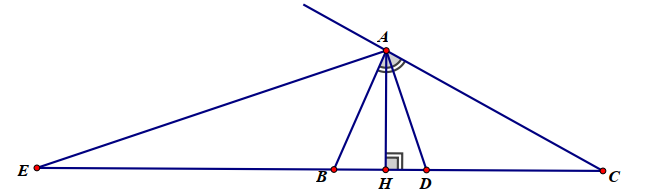
\includegraphics[width=0.65\textwidth]{3-4-lg.png}
    \begin{enumerate}
        \item $A D C=B+B A D \quad($ góc ngoài $\triangle \mathrm{ABD})(1)$\\
        $A D B=C+C A D$ ( góc ngoài $\triangle \mathrm{ADC})(2)$
        Mà $\mathrm{AD}$ là phân giác góc $\mathrm{BAD}$ nên $B A D=D A C(3)$\\
        Từ $(1),(2)$ và (3) suy ra đpcm
        \item
        Ta có:
        $$
        \begin{aligned}
        & A D C-A D B=B-C=40^{\circ} \\
        & A D C+A D B=180^{\circ} \\
        & \Rightarrow A D C=\frac{180^{\circ}+40^{\circ}}{2}=110^{\circ} ; A D B=70^{\circ} \\
        & \Rightarrow A H D=20^{\circ}
        \end{aligned}
        $$
        \item
        Ta có $\mathrm{AD}, \mathrm{AE}$ là hai tia phân giác của hai góc kê bù đỉnh $\mathrm{A}$ nên $\mathrm{AD} \perp \mathrm{AE}$\\
        Xét $\triangle \mathrm{AED} \quad$ ta có: $A E B+A D E=90^{\circ}$ (4)\\
        Xét $\triangle \mathrm{AHD}$ ta có: $H A D+A D E=90^{\circ}$ (5)\\
        Mặt khác\\
        $A D B=C+D A C=C+\frac{A}{2}$ \\
        $A+B+C=180^{\circ}$ \\
        $\Rightarrow \frac{A}{2}=90^{\circ}-\frac{B+C}{2}$ \\
        $A D B=C+90^{\circ}-\frac{B+C}{2}$ \\
        $\quad=\frac{C-B}{2}+90^{\circ}$ \\
        $\frac{\mathrm{B}-C}{2}+A D B=90^{\circ}(6)$\\
        Từ (4), (5) và (6) suy ra đpcm
    \end{enumerate}
}
\end{bt}

\begin{bt}
    \hfill
    \begin{enumerate}[a.]
        \item  Cho $S=1-\frac{1}{2}+\frac{1}{3}-\frac{1}{4}+\ldots+\frac{1}{2011}-\frac{1}{2012}+\frac{1}{2013}$ và $P=\frac{1}{1007}+\frac{1}{1008}+\ldots+\frac{1}{2012}+\frac{1}{2013}$.
        
        Tính $(S-P)^{2013}$.
        \item Cho $\mathrm{A}=\frac{\sqrt{x}+1}{\sqrt{x}-3}$
        
        Tìm $\mathrm{x} \in \mathrm{Z}$ để $\mathrm{A}$ có giá trị là một số nguyên.
    \end{enumerate}
\loigiai{
    \begin{enumerate}
        \item Ta có: \\
        $$
\begin{aligned}
& P=\frac{1}{1007}+\frac{1}{1008}+\ldots+\frac{1}{2012}+\frac{1}{2013} \\
& =\left(1+\frac{1}{2}+\frac{1}{3}+\ldots+\frac{1}{1006}+\frac{1}{1007}+\frac{1}{1008}+\ldots+\frac{1}{2012}+\frac{1}{2013}\right)-\left(1+\frac{1}{2}+\frac{1}{3}+\ldots+\frac{1}{1006}\right) \\
& =\left(1+\frac{1}{2}+\frac{1}{3}+\ldots+\frac{1}{1006}+\frac{1}{1007}+\frac{1}{1008}+\ldots+\frac{1}{2012}+\frac{1}{2013}\right)-2\left(\frac{1}{2}+\frac{1}{4}+\frac{1}{6}+\ldots+\frac{1}{2012}\right) \\
& =1-\frac{1}{2}+\frac{1}{3}-\frac{1}{4}+\ldots \ldots-\frac{1}{2012}+\frac{1}{2013}=S .
\end{aligned}
$$
Do đó $(S-P)^{2013}=0$
\item
Tìm $x \in z$ đề $A \in Z$
$$
\mathrm{A}=\frac{\sqrt{x}+1}{\sqrt{x}-3}=1+\frac{4}{\sqrt{x}-3} \quad(\mathrm{dk} \quad \mathrm{x} \geq 0, \mathrm{x} \neq 9)
$$
A nguyên khi $\frac{4}{\sqrt{x}-3}$ nguyên $\Rightarrow \sqrt{x}-3$ là Ư (4)
$$
\text{Ư}(4)=\{-4 ;-2 ;-1 ; 1 ; 2 ; 4\}
$$
Các giá trị của $x$ là : $1 ; 4 ; 16 ; 25 ; 49$.
    \end{enumerate}
}
\end{bt}